\documentclass[a4paper,12pt]{article}
\usepackage[T1]{fontenc}
\usepackage{imakeidx}
\usepackage{graphicx}
\begin{document}
\tableofcontents

\section{Introduction}
In this document,we spend some words on policies in IT \index{policies}, what is a policy, why we have them, and how many 

\clearpage

\section{What is a policy?}
A policy is a defined set of \emph{targets} every emploee in a \emph{company} has to try to achieve. Evidences proving the efforts to achieve the \emph{target} will be then recorded in some sort of document stored in a place every employee must be aware of. It's considered to be a \emph{statement of intent}. It is a commitment for every employee. The way to abide by the rules of a policy is essentially by showing one is doing the best possible to achieve the \emph{targets}. In every day practice it means spending reasonable effort to show the \emph{target} specified has been fairly achieved. You can label it they way you want and spend hours talking about it but it is essentially \textbf{common sense} written down black and white.
Every employee must be given a \emph{handbook} showing all the policies the company has to comply with.

\section{why we have them?}

Let's take for instance Environmental policies. The reason why we have them is because we might need to be able to deal with Minstery of Defence. Let's say one day a random employee, say \textbf{Giuseppe Mauro Maietta}, all of a sudden is being questioned by Ministery of Defence inspectors who went to check the company is really respecting the policies they have to abide with. If the employee knows what the policies are all about and knows where are they being kept then you have a happy ending, otherwise both the employer and the unlucky \textbf{Giuseppe Mauro Maietta} could be slapped with a huge fine. None of them will be happy, especially \textbf{Giuseppe} when eventually he will face prosecution with all unfortunate consequences. 

It's much better to know where the document is and what the policy is stating. That'll spare you from having to watch \textbf{Giuseppe} doing all sorts of gestures, shouting since he's perfectly aware he's going to get fired anyway.

People down there in Italy, they do all sort of things. You never know what to expect from them so knowing what a policy is, where is being kept is very much crucial indeed  


\section{Type of policies}
\subsection{Environmental policies}
This is a set of sort of good behaviours to follow to make sure the environment is respected. A company that wants to comply to these policies will have to have a saved set of records showing how much fuel are the trucks using and how much is the distance the trucks are covering. The problem is what the company is entitled to do might not always respect real scenario since what we can do is just see on google maps which one is the most convenient road for a truck to take but we cannot guarantee the truck really did that road. It's just to show we're doing what we need to protect the environment
\clearpage
\printindex

\section{examples}
\subsection{Sony Playstation Network Hacking}

Sony was attacked in the past and did warn that the names, addresses and other personal data of about 77 million people with accounts on its PlayStation Network (PSN) have been stolen.

Gamers have been locked out of the network for a week, but the company took one week to realize what was happening

Sony said it discovered that between 17 and 19 April an "illegal and unauthorised person" got access to people's names, addresses, email address, birthdates, usernames, passwords, logins, security questions and more. The PSN has been shutted down and players who were regular at Monster Hunter had to take a long break before they could face enemies like this again:

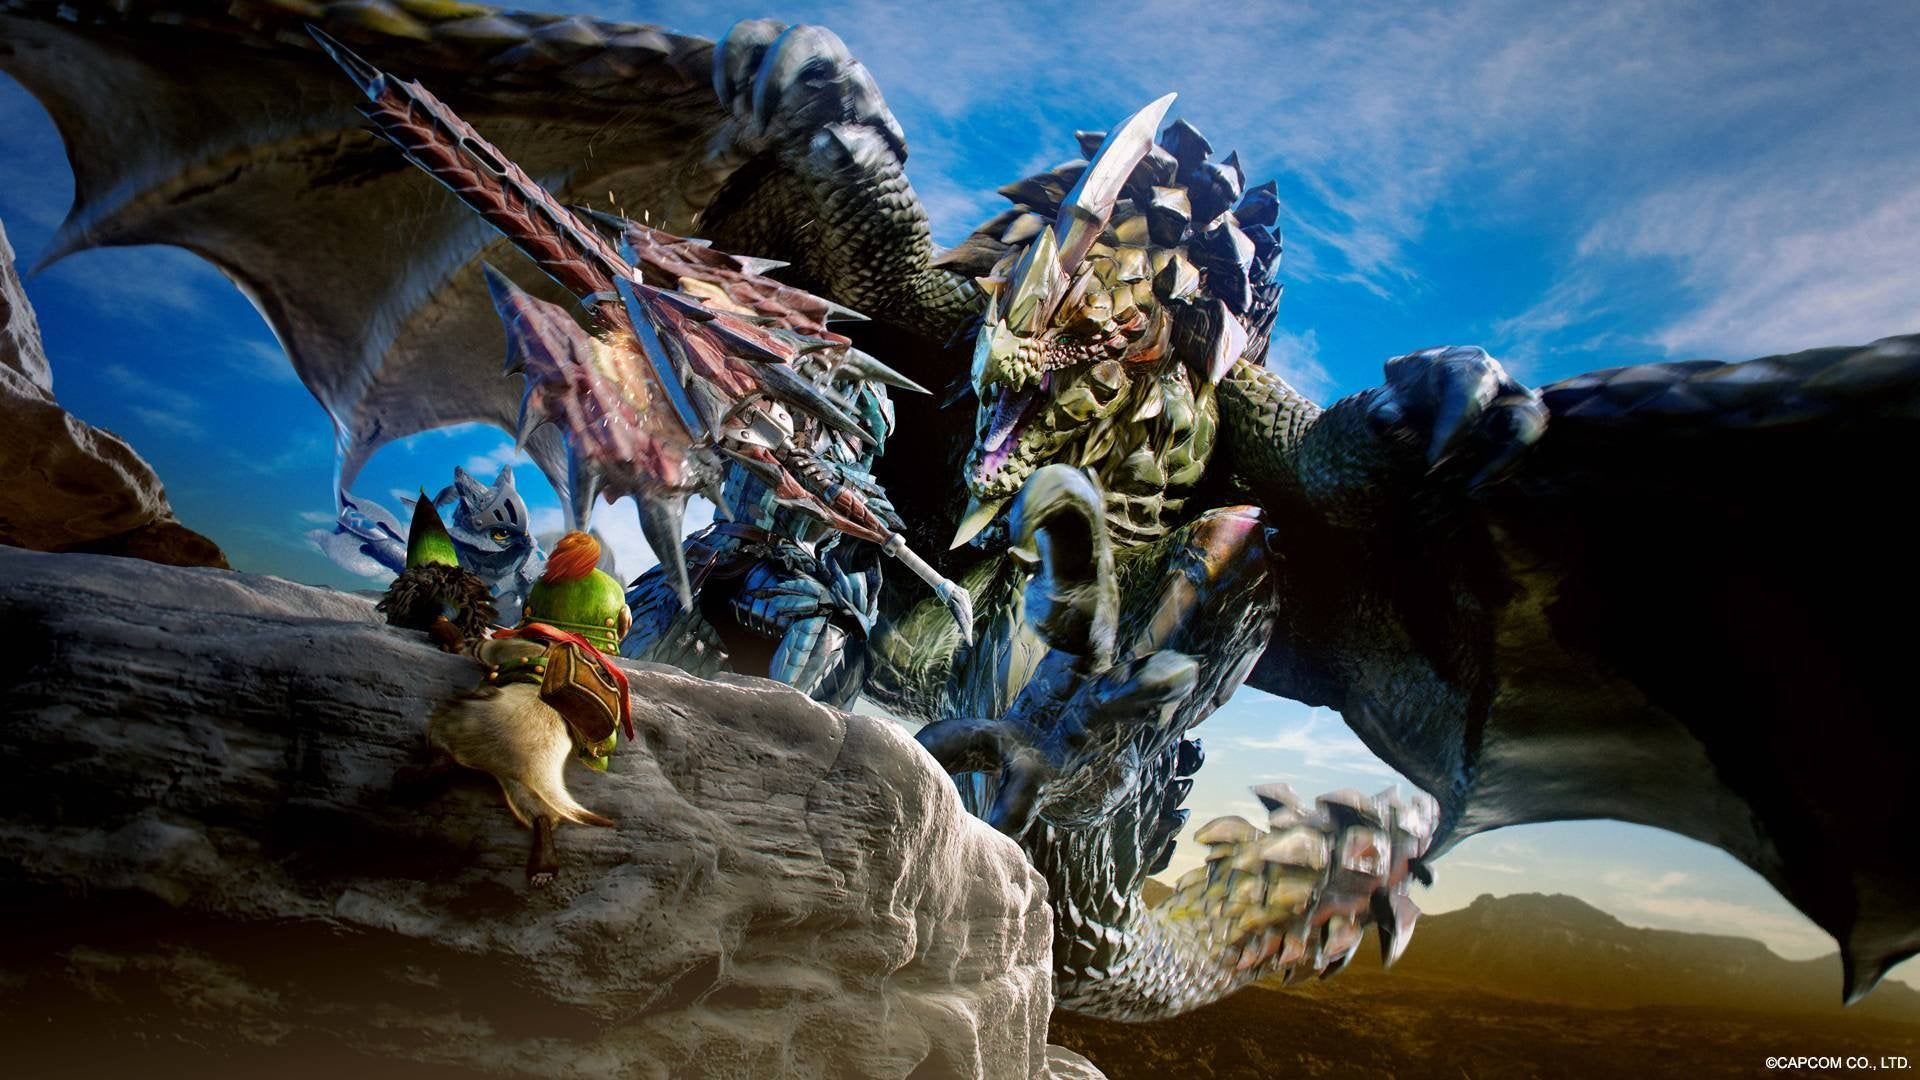
\includegraphics[width=15cm]{./seregios.jpg}

All gamers have been asked to sign lots of paperwork for free after which they have been rewarded with 3 games for free

But Sony upgraded its systems , announced it would finally introduce two-step verification, three years after Microsoft did the same for Xbox Live. There have been no widespread \emph{security breaches} since, although console networks remain vulnerable to concerted DDOS attacks - as seen when both PSN and Xbox Live failed over Christmas 2014.


\end{document}
